\section{Performance Discussion}\label{sec:experiments}

In this section, we evaluate the performance of the On-Demand
Checkpointing technique using an implementation of the proposed
approach in the \ompi framework. We first analyze the overheads and
performance in the \ompi implementation, then the performance of an
\abft QR operation implemented using On-Demand Checkpointing.

\subsection{MPI Fault Detection}

One of the concerns with fault tolerance is the amount of overhead
introduced by the fault tolerance management additions. Our
implementation of fault detection and propagation introduces very
little overhead to the MPI library. In the fault-free case, the
failure detection algorithm introduces no overhead as it is not
activated. It does introduce a small memory increase as the library
also needs to track the incarnation number of each process, however
this amount is relatively low as the incarnation number is only 8
bytes.

In the case where a fault occurs, the implementation is very efficient at
discovering the fault and propagating the information to the rest of the
application quickly. We performed a micro-benchmark a small local cluster as a
proof of concept. The cluster has 16 nodes with two 8-core Intel Xeon processors
each. We used only one core on each node because the increased number of ranks
on each core would not have an impact on the result of our measurements.

\begin{figure}[htb]
    \centering
    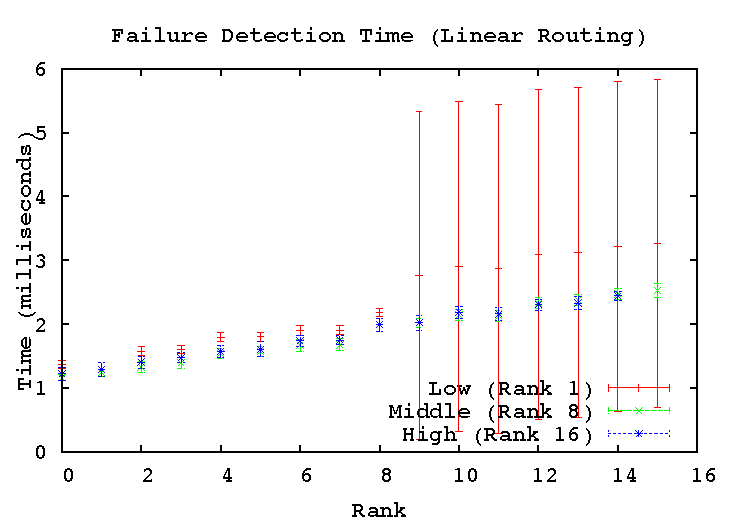
\includegraphics[width=0.4\textwidth]{figures/failure_detection_linear_errbars}
    \caption{Failure Detection and Propagation with a Linear Topology}
    \label{fig:linear}
\end{figure}

\begin{figure}[htb]
    \centering
    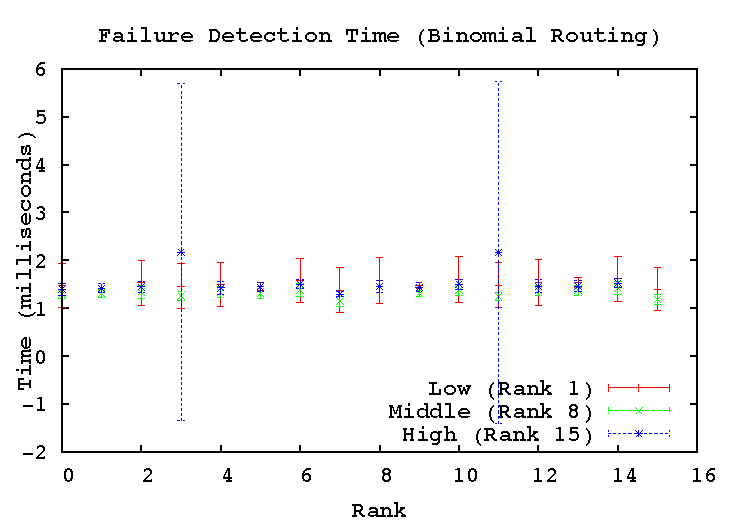
\includegraphics[width=0.4\textwidth]{figures/failure_detection_binomial_errbars}
    \caption{Failure Detection and Propagation with a Binomial Topology}
    \label{fig:binomial}
\end{figure}

Our evaluations used 16 nodes and ran 20 times for each test. The average value
is presented here. In the micro-benchmark, the code performs an MPI\_Barrier,
injects a failure at a specific rank, and then waits for a custom
MPI\_Errhandler to be called, alerting the MPI application to the process
failure. The time shown is the difference between the point directly before the
failure is injected and the moment the MPI\_Errhandler is called.
Figures~\ref{fig:linear} and~\ref{fig:binomial} show the time taken with two
communication topologies.  The linear topology in Figure~\ref{fig:linear} is a
simple topology where every node is connected to the HNP.
Figure~\ref{fig:binomial} shows a binomial tree topology. Because of the small
scale available to us, the failure propagation time is not effected by the
communication topology. We performed other tests on a larger machine, but due to
a machine specific issue, the results demonstrated too much noise to show useful
data. However, it did demonstrate that a tree-based topology can significantly
improve the communication time once the number of connections to the HNP would
overwhelm the linear communication pattern. Regardless of the small scale, these
results still acheive the goal of demonstrating the small amount of time
necessary to detect an propagate failures through the runtime.

This failure notification happens at the runtime system level,
asynchronously from any MPI call, ensures that with a high
probability, MPI processes will be notified of the failure during one
of the next MPI calls they enter. If the runtime system were not
propagating the failure notification, failures could be discovered by
MPI processes only when they try to communicate directly with a failed
process. Since in the On-Demande Checkpointing scheme, after they are
notified of a failure any process saves its state and then exits (thus
behaving as a failed process for the rest of the living processes),
all communicating processes would eventually be notified of the
initial failure. However, depending on the communication scheme of the
application, this notification using the in-band channels closure
could take significantly longer. Note that the \abft algorithm would
be able to recover from both scenarios. The out-of-band notification
of the runtime system is thus there to improve the performance by
reducing the latency needed to enter the recovery procedure.

% WE SHOULD HAVE SOME RESULTS WITH AUTO-FT AND/OR APP BASED PERIODIC CHECKPOINT


\subsection{On-Demand Checkpointing for QR}
The On-Demand Checkpointing QR checkpoints data from memory 
to disk on the living processes at the time of failure. Therefore 
disk I/O access time is a critical component of the performance overhead. 

To evalue the performance impact of disk access, the implenentation of the
On-Demand Checkpointing algorithm based on the ScaLAPACK QR is tested
on two cluster systems at different scale. The first machine,
``Dancer'', is a 16-node cluster at the University of Tennessee,
Knoxville. All nodes are equipped with two 2.27GHz quad-core Intel
E5520 CPUs, connected by 20GB/s Infiniband. Solid State Drive disks
are used as the checkpoint storage media.  The second system is the
Kraken supercomputer by Cray Inc. at the Oak Ridge National Lab.
Kraken has 9,408 compute nodes. Each node has two Istanbul 2.6 GHz
six-core AMD Opteron processors, 16 GB of memory, and a highly
scalable cluster file system ``Lustre''.  All the nodes are Connected
by the Cray SeaStar2+ interconnect.  In all experiments, the block
size is set to 100.

\begin{figure}[tb]
	\centering
	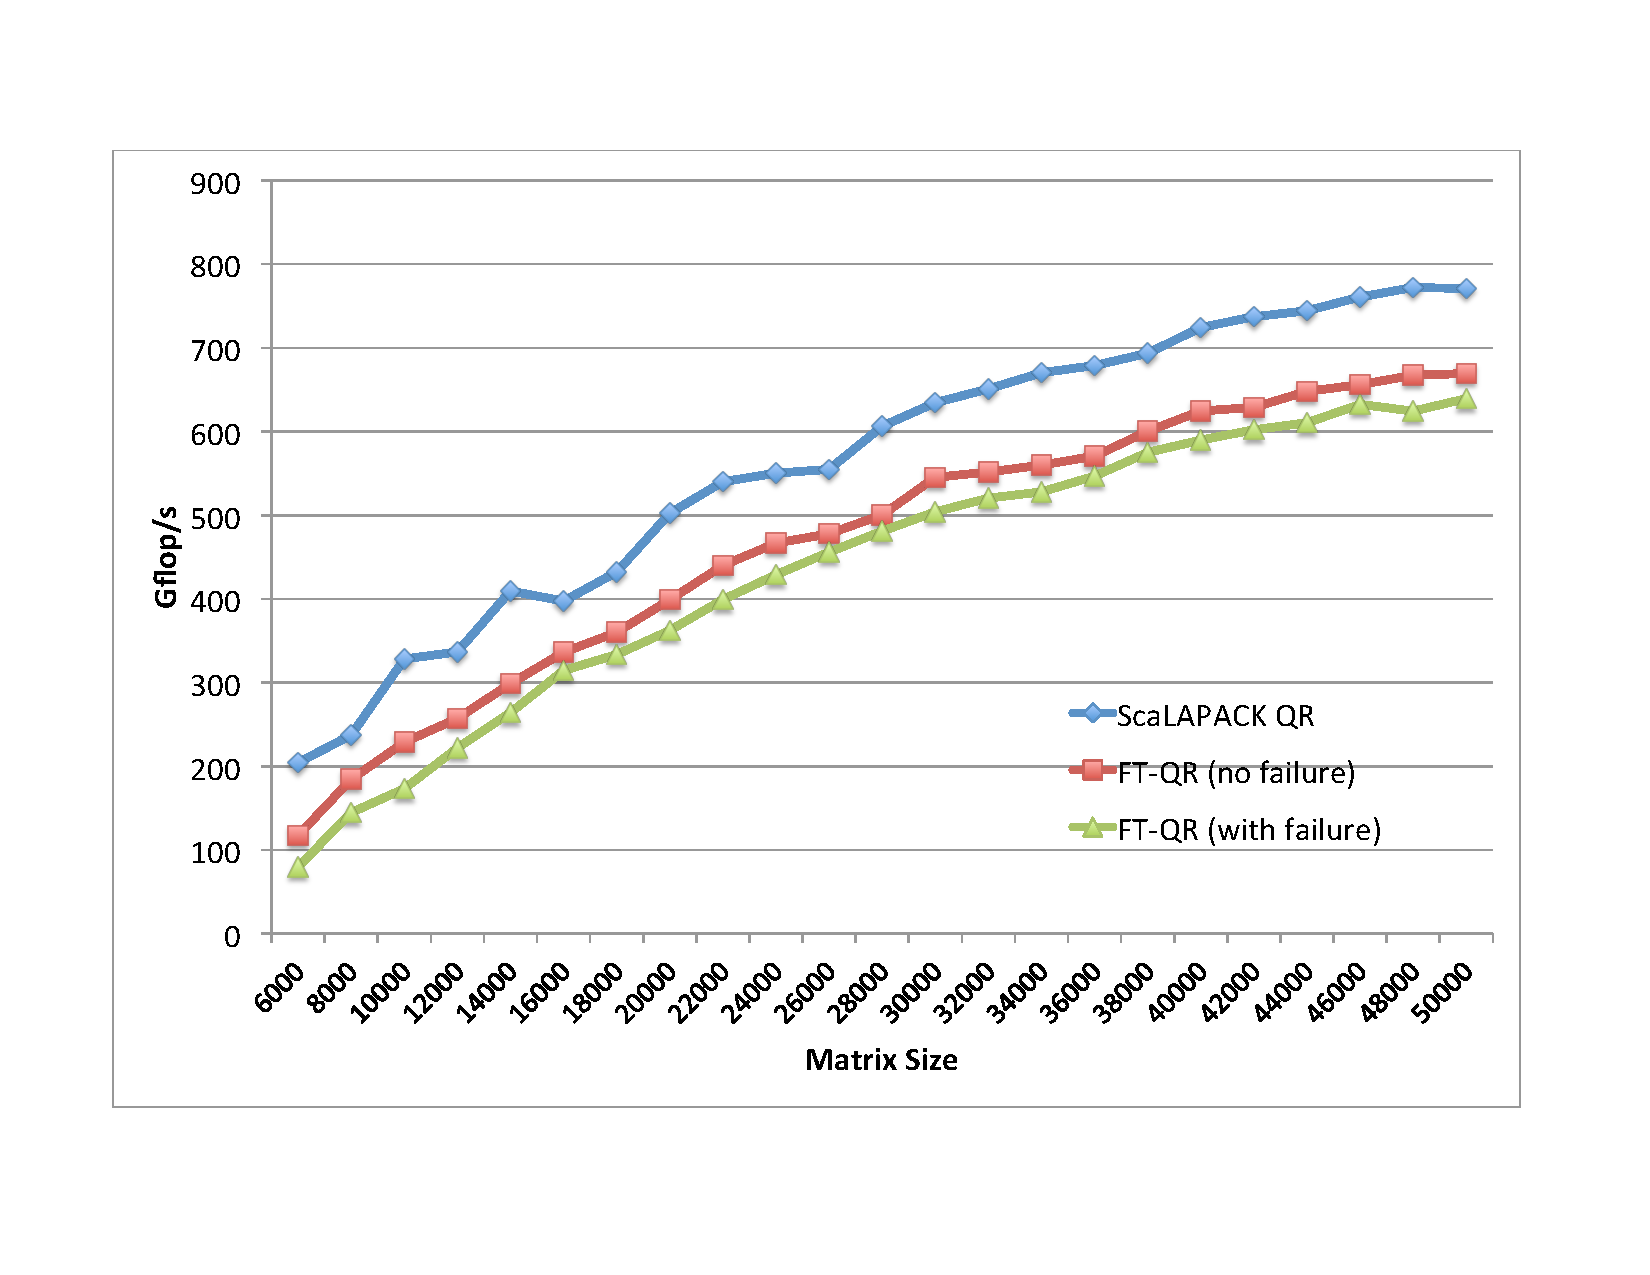
\includegraphics[totalheight=0.25\textheight, width=0.45\textwidth,viewport=70 90 720 530, clip]{figures/dancer_performance}
	\caption{Performance on Dancer ($16\times 8$ grid)}
	\label{fig:dancer_performance}
\end{figure}


Figure~\ref{fig:dancer_performance} presents the performance of this
QR implementation on the Dancer cluster with a $8\times 16$ process
grid.  The FT-QR (no failure) presents the performance of the
On-Demand Checkpointing implementation, in a fault-free execution,
while the FT-QR (with failure) curves present the performance of the
same implemenation, when the failure is injected after the first step
of PDLARFB that performs $W\leftarrow V^{T}A_{2}$. The performance
of the non-fault tolerant ScaLAPACK QR is also presented to
serve as a reference.

The difference with the ScaLAPACK QR is caused by the parallel-Q
checksum and the \abft algorithm. This overhead has been shown
in~\cite{lawn253} to scale down with larger number of processes and
matrices. In the case of a run with an error, the following overheads
adds up: the times to store the checkpoint to disk, re-launch an
application, re-establish the position of all processes by dry running
in the application until the failing point, loading checkpoint from
disk and perform the \abft recovery using the checksum found in the
checkpoint of the previously living processes. 

On Dancer, the performance of QR with on-demand checkpointing and
recovery follows closely with the ``no failure''
performance. Figure~\ref{fig:dancer_percentage} shows that as the
matrix size increases, the recovery overhead falls below 5\% more than
the ``no failure'' overhead. By breaking down the run-time of each
recovery elements, Figure~\ref{fig:dancer_timing} shows that
checkpoint saving and loading only take a small percentage of the
total run-time.  On a problem of this size, the additional overheads
are dominated by the time it takes to terminate the failing MPI
application and relaunch a new one. Other than the fast solid state
drive disks, the fast checkpointing can also be attributed to the disk cache
provided by the OS. Since loading is performed
immediately after saving, high disk cache hits can
largely speed up the process. After matrix size 44,000 the memory
usage on each node came close to limit and since no swap space is 
available on the Dancer cluster, disk cache support started
to decrease and cause slight increase in disk access time, which however does not
affect the overhead percentage from performing recovery. 

\begin{figure}[tb]
	\centering
	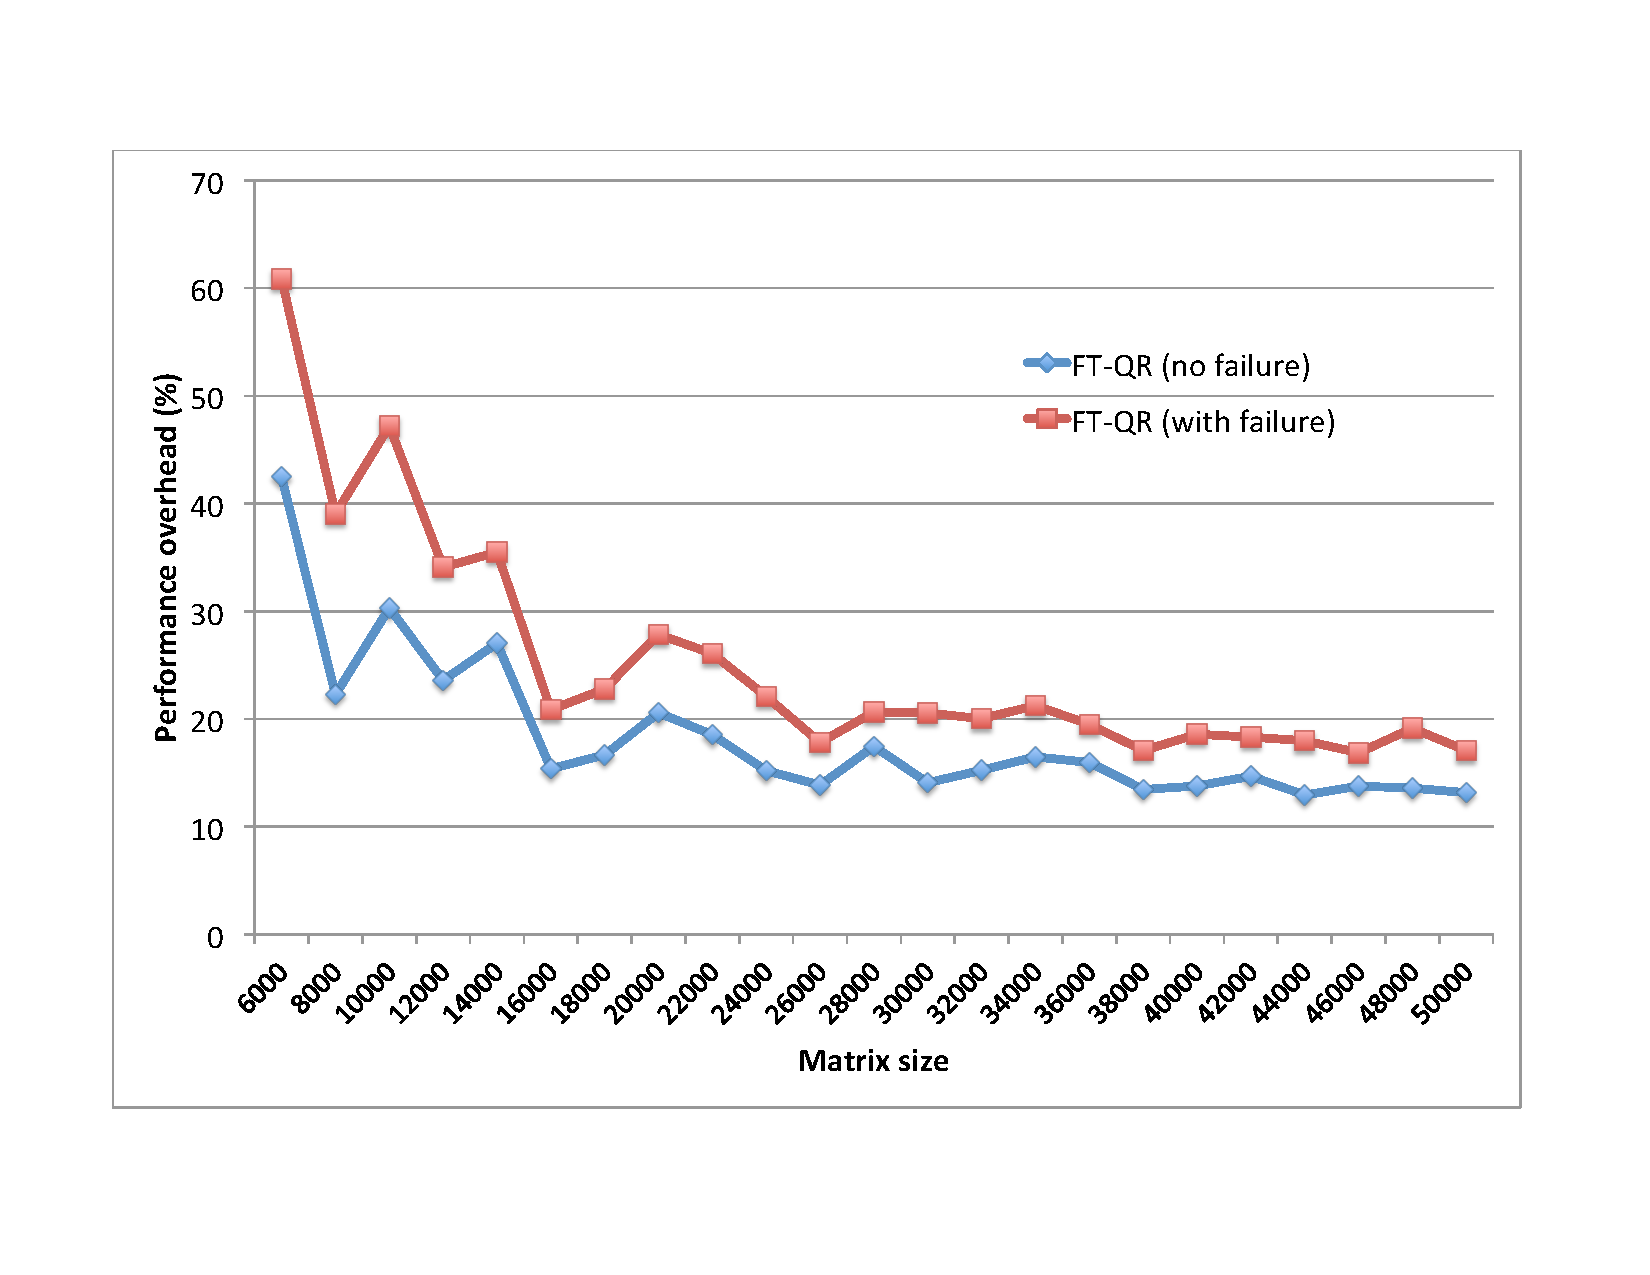
\includegraphics[totalheight=0.25\textheight, width=0.45\textwidth,viewport=70 90 720 530, clip]{figures/dancer_percentage}
	\caption{Overhead over ScaLAPACK QR on Dancer ($16\times 8$ grid)}
	\label{fig:dancer_percentage}
\end{figure}

Figure~\ref{fig:kraken_performance} presents the performance on Kraken
with a larger grid and a different filesystem to store the checkpoint
images. A similar effect of a small checkpointing saving and loading
time is observed. The performance of the ``with failure'' case shows
the same trend of closely following the ``no failure'' case
performance. At size matrix 100,000 for instance, FT-QR successfully recovered from
the failure and achieved 2.86 Tflop/s, which is 90\% of the
performance of the ScaLAPACK QR.  This verified that the On-Demand
Checkpointing QR also performs well at larger scales.

\begin{figure}[b]
	\centering
	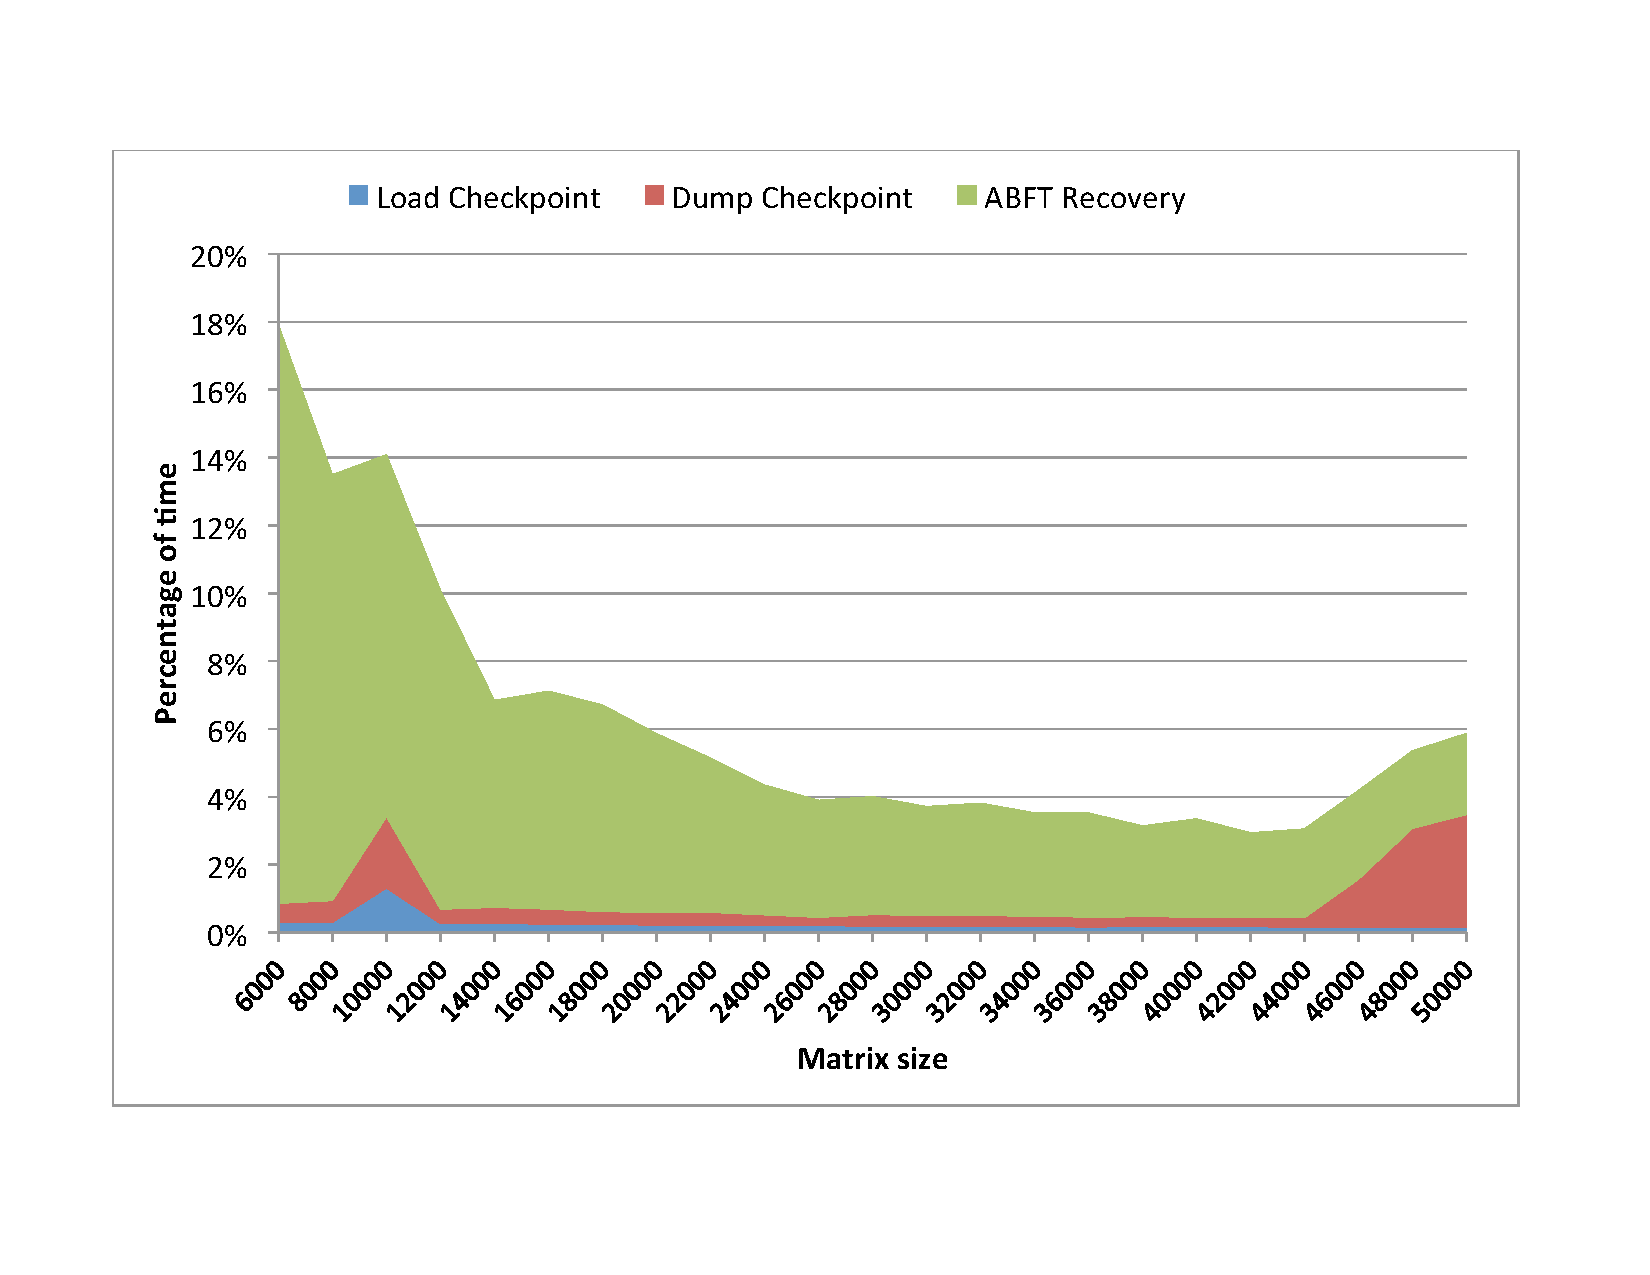
\includegraphics[totalheight=0.25\textheight, width=0.45\textwidth,viewport=70 90 720 530, clip]{figures/dancer_1_error_timing_process_new}
	\caption{Time Breakdown of FT-QR on Dancer ($16\times 8$ grid)}
	\label{fig:dancer_timing}
\end{figure}

\begin{figure}[t]
	\centering
	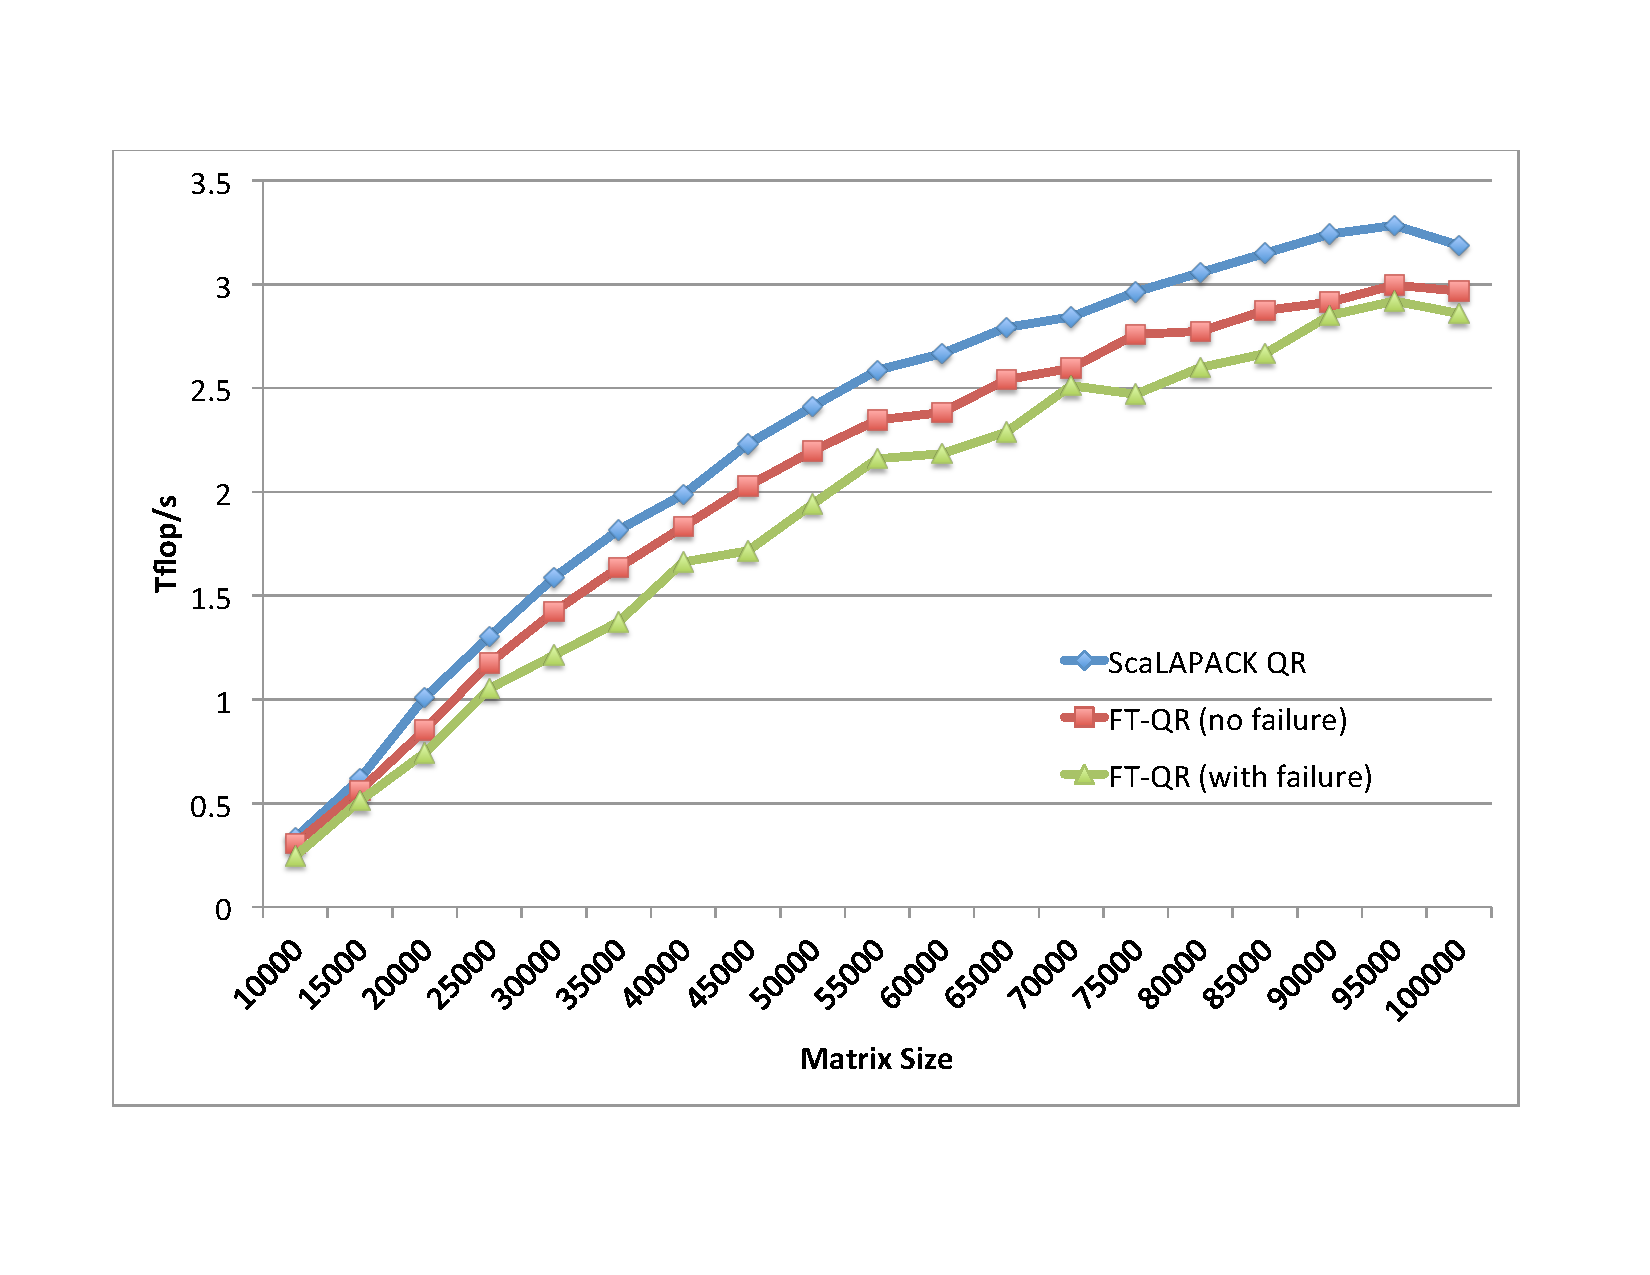
\includegraphics[totalheight=0.25\textheight, width=0.45\textwidth,viewport=70 90 720 530, clip]{figures/kraken_new}
	\caption{Performance on Kraken ($24\times 24$ grid)}
	\label{fig:kraken_performance}
\end{figure}
